\documentclass[thesis.tex]{subfiles}
\begin{document}
\chapter{Modeling and Evaluation of Sentence Simplification}
\label{chap:sentence}

\section{Introduction}
In the previous chapter, we focused on complex words, and their substitution with simpler words that preserve the original in-context meaning. In this chapter, we instead consider the task of simplifying an entire sentence, a task known as sentence simplification. Most recent sentence simplification research has approached this task as a monolingual machine translation problem, where the goal is to transform a complex English sentence into a simpler sentence that preserves the meaning of the original sentence \citep{zhu2010monolingual,narayan2014hybrid}. 

This chapter includes two sections. In the first section, we consider applying sequence-to-sequence (Seq2Seq) models to the task of sentence simplification, and propose various modifications to extend the generic framework during training, inference, and post-inference. We also provide an extensive error analysis to show where current sentence simplification models fall short. In the second section, we discuss how to fine-tune a BERT-based model on fluency, adequacy, and complexity simultaneously in order to predict the overall quality of sentence simplification system output without the need for references.

\section{Complexity-Weighted Loss and Diverse Re-Ranking for Sentence Simplification} \label{sec:sentence}

If we frame simplification as a monolingual translation problem, a natural approach is to follow a machine translation approach and apply sequence-to-sequence (Seq2Seq) models  \citep{sutskever2014sequence,luong2015effective,vaswani2017attention}. Seq2Seq models learn mappings from one sequence to another using a neural network, and have shown state-of-the-art performance on other related monolingual natural language processing generation tasks, including text summarization \citep{nallapati2016abstractive} and dialog systems \citep{vinyals2015neural}. 

One of the main limitations in applying standard Seq2Seq models to simplification is that these models tend to copy directly from the original complex sentence too often, as this is the most common operation in simplification. Several recent efforts have attempted to alleviate this problem using reinforcement learning \citep{zhang2017sentence} and memory augmentation \citep{zhao2018integrating}, but these systems often still produce outputs that are longer than the reference sentences. To avoid this problem, we propose to extend the generic Seq2Seq framework at both training and inference time by encouraging the model to choose simpler content words, and by effectively choosing an output based on a large set of candidate simplifications. The main extensions from this work can be summarized as follows:

\begin{itemize}
    \item We propose a custom loss function to replace standard cross entropy probabilities during training, which takes into account the complexity of content words.
    \item We include a similarity penalty at inference time to generate more diverse simplifications, and we further cluster similar sentences together to remove highly similar candidates.
    \item We develop methods to re-rank candidate simplifications to promote fluency, adequacy, and simplicity, helping the model choose the best option from a diverse set of sentences.
\end{itemize}

An analysis of each individual components reveals that of the three contributions, re-ranking simplifications at post-decoding stage brings about the largest benefit for the simplification system. We compare our model to several state-of-the-art systems in both an automatic and human evaluation settings, and show that the generated simple sentences are shorter and simpler, while remaining competitive with respect to fluency and adequacy. We also include a detailed error analysis to explain where the model currently falls short and provide suggestions for addressing these issues.

\subsection{Seq2Seq Approach}

\subsubsection{Complexity-Weighted Loss Function} \label{loss}

Standard Seq2Seq models use cross entropy as the loss function at training time. This only takes into account how similar our generated tokens are to those in the reference simple sentence, and not the complexity of said tokens. Therefore, we first develop a model to predict word complexities, and incorporate these into a custom loss function.

Extending the binary complex word identification model from Chapter \ref{chap:lexical}, we train a linear regression model using length, number of syllables, and word frequency; we also include Word2Vec embeddings \citep{mikolov2013distributed}. We leverage the Newsela corpus to collect data for this task by extracting word counts in each of the five reading levels, labeling each word with a complexity level based on those counts. We propose using Algorithm \ref{alg:word-complexity} to obtain the complexity label for each word $w$, where $l_w$ represents the level given to the word, and $c_{w_i}$ represents the number of times that word occurs in level $i$.

\begin{algorithm}
\caption{Word Complexity Data Collection}
\label{alg:word-complexity}

\begin{algorithmic}[1]
\Procedure{Data Collection}{}
\State $l_w \gets 4$ 
\For{$i \in \{3, 0\}$}
    \If{$c_{w_i} \geq 0.7*c_{w_{i+1}}$}
        \If{$c_{w_i} \geq 0.4*c_{w_4}$}
            \State $l_w \gets i$
        \EndIf
    \EndIf
\EndFor

\Return $l_w$
\EndProcedure
\end{algorithmic}
\end{algorithm}

Here, we initially label the word with the most complex level, 4. If at least 70\% of the instances of this word is preserved in level 3, we reassign the label as level 3; if the label was changed, we then do this again for progressively simpler levels. As examples, Algorithm \ref{alg:word-complexity} labels ``pray", ``sign", and ``ends" with complexity level 0, and ``proliferation", ``consensus", and ``emboldened" with complexity level 4. We split the data extracted from Algorithm \ref{alg:word-complexity} into Train, Validation and Test sets (90\%, 5\% and 5\%, respectively, and use them for training and evaluating the complexity prediction model. Note that we also tried continuous rather than discrete labels for words by averaging frequencies, but found that this increased the noise in the data. For example, ``the" and ``dog" were incorrectly labeled as level 2 instead of 0, since these words are seen frequently across all levels.

\begin{table}
\begin{center}
\begin{tabular}{|c|c|cccccc|} \hline \multirow{2}{*}{\textbf{Model}} & \multirow{2}{*}{\textbf{Correlation}} & \multicolumn{6}{c|}{\textbf{Mean Squared Error}} \\
& & \textbf{Overall} & \textbf{0} & \textbf{1} & \textbf{2} & \textbf{3} & \textbf{4} \\ \hline
Frequency & -0.031 & 1.9 & 2.24 & 0.38 & 0.64 & 3.01 & 6.99\\
Length & 0.344 & 1.51 & 1.03 & \textbf{0.32} & 0.89 & 2.95 & 6.90 \\
LinReg & \textbf{0.659} & \textbf{0.92} & \textbf{0.92} & 0.39 & \textbf{0.49} & \textbf{1.17} & \textbf{3.27} \\ \hline
\end{tabular}
\end{center}
\caption{\label{word-comp} Pearson Correlation, Overall Mean Squared Error (MSE), and MSE by complexity level for our word-level complexity prediction model. We compare to length-based and frequency-based baselines.}
\end{table}

We report the Mean Squared Error (MSE) and Pearson correlation on our test set in Table \ref{word-comp}. We compare our model (LinReg) to the two strongest baselines from Chapter \ref{chap:lexical}, which predict complexity using log Google $n$-grams frequency \citep{thorsten2006web} and word length, respectively.

Once we have a reliable way of making word-level complexity predictions, we then propose a method that modifies cross entropy loss to up-weight simple words while down-weighting more complex words. More formally, the probabilities of our simplified loss function can be generated by the process described in Algorithm \ref{alg:loss-function}. Since our word complexities are originally from 0 to 4, with 4 being the most complex, we need to reverse this ordering and add one, so that more complex words and non-content words are not given zero probability. In this algorithm, we denote the original probability vector as \textbf{CE}, our vocabulary as $\textbf{V}$, the predicted word complexity of a word $v$ as $score_v$, the resulting weight for a word as $w_v$, and our resulting weights as \textbf{SCE}, which we then normalize and convert back to logits.

\begin{algorithm}
\caption{Simplified Loss Function}
\label{alg:loss-function}

\begin{algorithmic}[1]
\Procedure{Simplified Loss}{}
\State $\textbf{CE} \gets$ softmax($logits_{CE}$)
\For{$v \in \textbf{V}$}
    \State $score_v \gets WordComplexity(v)$
    \If{$v$ is a content word}
        \State $w_v \gets (4 - s_v) + 1$
    \Else
        \State $w_v \gets 1$
    \EndIf
\EndFor
\State $w_v \gets \Big(\frac{w_v}{\sum_{v\in V}w_v}\Big)^{\alpha}$ for $v \in \textbf{V}$
\State $\textbf{SCE} \gets \textbf{CE} \cdot \textbf{w}$

\Return $\textbf{SCE}$
\EndProcedure
\end{algorithmic}
\end{algorithm}

Here, $\alpha$ is a parameter we can tune during experimentation.
Note that we only upweight simple content words, not stopwords or entities.

\subsubsection{Diverse Candidate Simplifications} \label{sec:sentence_diverse}

To increase the diversity of our candidate simplifications, we apply a beam search scoring modification proposed in \cite{li2016simple}. In standard beam search with a beam width of $b$, given the $b$ hypotheses at time $t-1$, the next set of hypotheses is generated by first selecting the top $b$ candidate expansions from each hypothesis. These $b\times b$ hypotheses are then ranked by the joint probabilities of their sequence of output tokens, and the top $b$ according to this ranking are chosen.

We observe that candidate expansions from a single parent hypothesis tend to dominate the search space over time, even with a large beam. To increase diversity, we apply a penalty term based on the rank of a generated token among the $b$ candidate tokens from its parent hypothesis.

If $Y^j_{t-1}$ is the $j^{th}$ top hypothesis at time $t-1$, $j\in[1..b]$, and $y_t^{j,j'}$ is a candidate token generated from $Y^j_{t-1}$, where $j'\in[1..b]$ represents the rank of this particular token among its siblings, then our modified scoring function is as follows (here, $\delta$ is a parameter we can tune during experimentation):
\begin{equation}
\small
S(Y_{t-1}^j,y_t^{j,j'})=\log{p(y_1^j,\dots,y_{t-1}^j,y_t^{j,j'}|x)}-j'*\delta
\end{equation}

Extending the work of \cite{li2016simple}, to further increase the distance between candidate simplifications, we can cluster similar sentences after decoding. To do this, we convert each candidate into a document embedding using Paragraph Vector \citep{le2014distributed}, cluster the vector representations using $k$-means, and select the sentence nearest to the centroids. This allows us to group similar sentences together, and only consider candidates that are relatively more different. Note that this is only one of many possible diverse decoding approaches, I explore these in more detail in Chapter \ref{chap:decoding_strategies}.

\subsubsection{Re-ranking Diverse Candidates}

Generating diverse sentences is helpful only if we are able to effectively re-rank them in a way that promotes simpler sentences while preserving fluency and adequacy. To do this, we propose three ranking metrics for each sentence $i$:

\begin{itemize}
    \item \textbf{Fluency} ($f_i$): We calculate the perplexity based on a 5-gram language model trained on English Gigaword v.5 \citep{parker2011english} using KenLM \citep{heafield2011kenlm}.
    \item \textbf{Adequacy} ($a_i$): We generate Paragraph Vector representations \cite{le2014distributed} for the input sentence and each candidate and calculate the cosine similarity.
    \item \textbf{Simplicity} ($s_i$): We develop a sentence complexity prediction model to predict the overall complexity of each sentence we generate.
\end{itemize}

To calculate sentence complexity, we modify a Convolutional Neural Network (CNN) for sentence classification \citep{kim2014convolutional} to make continuous predictions. We use aligned sentences from the Newsela corpus \citep{xu2015problems} as training data, labeling each with the complexity level from which it came. We normalize each individual score between 0 and 1, and calculate a final score as follows:

\begin{equation}
    score_i = \beta_ff_i + \beta_aa_i + \beta_ss_i
\end{equation}

We tune these weights (\textbf{$\beta$}) on our validation data during experimentation to find the most appropriate combinations of re-ranking metrics.

\subsection{Experiments} \label{sec:sentence_experiments}

We train our models on the Newsela Corpus \citep{xu2015problems}. Following \cite{zhang2017sentence}, we exclude sentence pairs corresponding to levels 4-3, 3-2, 2-1, and 1-0, where the simple and complex sentences are just one level apart, as these are too close in complexity. After this filtering, we are left with 94,208 training, 1,129 validation, and 1,077 test sentence pairs; these splits are the same as \cite{zhang2017sentence}. We preprocess our data by tokenizing and replacing named entities using CoreNLP \citep{manning2014stanford}. 

For our experiments, we use Sockeye, an open source Seq2Seq framework built on Apache MXNet \citep{hieber2017sockeye,chen2015mxnet}. In this model, we use LSTMs with attention for both our encoder and decoder models. We attempt to match the hyperparameters described in \cite{zhang2017sentence} as closely as possible; as such, we use 300-dimensional pretrained GloVe word embeddings \citep{pennington2014glove}, and Adam optimizer \citep{kingma2015adam}. Table \ref{tab:params} shows a comprehensive list of all hyperparameters we used when training our default Seq2Seq model. This list includes learning rate (LR), learning rate reduction rate (LR reduce), size of embeddings (Embeddings), loss function (loss, we use CE to represent Cross Entropy), among others. 

\begin{table}
\small
\begin{center}
\begin{tabular}{|c|c|c|c|} \hline
\textbf{Parameter} & \textbf{Value} & \textbf{Parameter} & \textbf{Value} \\ 
\hline
Batch size & 86 & Embeddings & 300:300\\
RNN hidden units & 256 & LR & 0.001\\
RNN attention & dot & LR reduce & 0.7\\
\# of layers & 2 & Loss & CE\\
RNN type & LSTM & Min Epochs & 1\\
Dropout inputs & 0.2 & Max epochs & 30\\
Dropout states & 0.2 & Max updates & 500000\\
Min vocab freq & 3 & \# Last params & 5\\
Max length & 85 & Optimizer & Adam\\
Label smoothing & 0 & Seed & 13\\
\hline
\end{tabular}
\end{center}
\caption{\label{tab:params} Training Hyperparameters for the baseline Seq2Seq model and our extended model.}
\end{table}

For our extensions to the standard Seq2Seq framework, we use nearly all the same parameters, the only exception being that we change the loss function from cross entropy to our custom complexity-weighted loss function. With this loss, we use $\alpha = 2$ during training. At inference time, we set the beam size $b = 100$, and the similarity penalty $d = 1.0$. After inference, we set the number of clusters to 20, and we compare two separate re-ranking weightings: one which uses fluency, adequacy, and simplicity (FAS), where $\beta_f = \beta_a = \beta_s = \frac{1}{3}$; and one which only uses fluency and adequacy (FA), where $\beta_f = \beta_a = \frac{1}{2}$ and $\beta_s$ = 0. Note that our best model uses FA weights.

We compare our models to the following baselines:

\begin{itemize}
    \item \textbf{Hybrid} performs sentence splitting and deletion before simplifying with a phrase-based machine translation system \citep{narayan2014hybrid}.
    \item \textbf{DRESS} is a Seq2Seq model trained with reinforcement learning which integrates lexical simplifications \citep{zhang2017sentence}.\footnote{For Hybrid and DRESS, we use the generated outputs provided in \cite{zhang2017sentence}. We made a significant effort to rerun the code for DRESS, but were unable to do so.}
    \item \textbf{DMASS} is a Seq2Seq model which integrates the transformer architecture and additional simplifying paraphrase rules \citep{zhao2018integrating}.\footnote{For DMASS, we ran the authors' code on our data splits from Newsela, in collaboration with the first author to ensure an accurate comparison.}
\end{itemize}

We also present results on several variations of our models, to isolate the effect of each individual improvement. \textbf{Seq2Seq} is a standard sequence-to-sequence model with attention and greedy search. \textbf{Seq2Seq-Loss} is trained using our complexity-weighted loss function and greedy search. \textbf{Seq2Seq-FA} uses beam search, where we re-rank all sentences using fluency and adequacy (FA weights). \textbf{Seq2Seq-Cluster-FA}  clusters the sentences before re-ranking using FA weights. \textbf{Seq2Seq-Diverse-FA} uses diversified beam search, re-ranking using FA weights. \textbf{Seq2Seq-All-FAS} uses all contributions, re-ranking using fluency, adequacy, and simplicity (FAS weights). Finally, \textbf{Seq2Seq-All-FA} integrates all modifications we propose, and re-ranks using FA weights.

Following previous work \citep{zhang2017sentence,zhao2018integrating}, we use SARI as our main automatic metric for evaluation \citep{xu2016optimizing}.\footnote{To compute SARI, we use the original script provided by \citep{xu2016optimizing}.} SARI calculates how often a generated sentence correctly keeps, inserts, and deletes $n$-grams from the complex sentence, using the reference simple sentence as the gold-standard, where $1 \leq n \leq 4$. We also calculate oracle SARI, where appropriate, to show the score we could achieve if we had a perfect re-ranking model. Our results are reported on the left side of Table \ref{tab:sent_auto}.

Our best models outperform previous state-of-the-art systems, as measured by SARI. When used separately, re-ranking and clustering results in the largest improvements on this metric. Our loss and diverse beam search methods have more ambiguous effects, especially when combined with the former two; note however that including diversity before clustering does slightly improve the oracle SARI score.

\begin{table}
\begin{center}
\small
\begin{tabular}{|l|cc|ccccc|} \hline
\textbf{Model} & \textbf{SARI} & Oracle & \textbf{Len} & \textbf{FKGL} & \textbf{TER} & \textbf{Ins} & \textbf{Edit}\\ \hline
Complex & -- & -- & 23.1 & 11.14 & 0 & 0 & -- \\ \hline
Hybrid & 33.27 & -- & 12.4 & 7.82 & 0.49 & 0.01 & --\\
DRESS & 36.00 & -- & 14.4 & 7.60 & 0.44 & 0.07 & --\\ 
DMASS & 34.35 & -- & 15.1 & 7.40 & 0.59 & 0.28 & -- \\ \hline
Seq2Seq & 36.32 & -- & 16.1 & 7.91 & 0.41 & 0.23 & -- \\
Seq2Seq-Loss & 36.03 & -- & 16.4 & 8.11 & 0.40 & \textbf{0.31} & --\\
Seq2Seq-FA & 36.47 & 54.01 & 7.6 & 6.42 & 0.73 & 0.01 & 7.28 \\
{\scriptsize Seq2Seq-Cluster-FA} & \textbf{37.22} & 50.36 & 9.1 & 6.49 & 0.68 & 0.05 & 7.55 \\
{\scriptsize Seq2Seq-Diverse-FA} & 35.36 & 52.65 & 7.5 & 5.97 & \textbf{0.78} & 0.07 & \textbf{8.22} \\
Seq2Seq-All-FAS & 36.30 & 50.40 & 9.1 & \textbf{5.37} & 0.68 & 0.05 & 7.56 \\
Seq2Seq-All-FA & 37.11 & 50.40 & 10.8 & 6.42 & 0.61 & 0.07 & 7.56 \\ \hline
Reference & 100 & -- & 12.8 & 6.90 & 0.67 & 0.42 & --\\
\hline
\end{tabular}
\end{center}
\caption{\label{tab:sent_auto} Comparison of our models to baselines and state-of-the-art models using SARI. We also include oracle SARI scores (Oracle), given a perfect re-ranker. Seq2Seq-All-FA is significantly better than the baselines using a student t-test ($p < 0.05$). We also calculate average sentence length, FKGL, TER score compared to input, number of insertions, and average edit distance (Edit) between candidate sentences for applicable models.}
\end{table}

We calculate several descriptive statistics on the generated sentences and report the results on the right side of Table \ref{tab:sent_auto}. We observe that our models produce sentences that are much shorter and lower reading level, according to Flesch-Kincaid grade level (FKGL) \citep{kincaid1975derivation}, while making more changes to the original sentence, according to Translation Error Rate (TER) \citep{snover2006study}. In addition, we see that the customized loss function increases the number of insertions made, while both the diversified beam search and clustering techniques individually increase the distance between sentence candidates.

While SARI has been shown to correlate with human judgments on simplicity, it only weakly correlates with judgments on fluency and adequacy \citep{xu2016optimizing}. Furthermore, SARI only considers simplifications at the word level, while we believe that a simplification metric should also take into account sentence structure complexity.

Due to limitations of current automatic metrics, we also choose to elicit human judgments on 200 randomly selected sentences to determine the relative overall quality of our simplifications. For our first evaluation, we ask native English speakers on Amazon Mechanical Turk to evaluate the fluency, adequacy, and simplicity of sentences generated by our systems and the baselines, similar to \cite{zhang2017sentence}. Each annotator rated these aspects on a 5-point Likert Scale. These results are found in Table \ref{tab:sent_human}.

\begin{table*}
\begin{center}
\begin{tabular}{|l|cccc|}
\hline
\textbf{Model} & \textbf{Fluency} & \textbf{Adequacy} & \textbf{Simplicity} & \textbf{All} \\ \hline
Hybrid & 2.79* & 2.76 & 2.88* & 2.81* \\
DRESS & \textbf{3.50} & \textbf{3.11}* & 3.03 & \textbf{3.21}* \\ 
DMASS & 2.59* & 2.15* & 2.50* & 2.41* \\ \hline
Seq2Seq-All-FAS & 3.35 & 2.50* & \textbf{3.11} & 2.99 \\
Seq2Seq-All-FA & 3.38 & 2.66 & \textbf{3.08} & 3.04 \\ \hline
Reference & 3.82* & 3.23* & 3.29* & 3.45* \\ \hline
\end{tabular}
\end{center}
\caption{\label{tab:sent_human} Average ratings of crowdsourced human judgments on fluency, adequacy and complexity. Ratings significantly different from Seq2Seq-All-FA are marked with * ($p < 0.05$); statistical significance tests were calculated using a student t-test. We provide 95\% confidence intervals for each rating in the appendix.}
\end{table*}

As we can see, our best models substantially outperform the Hybrid and DMASS systems. Note that DMASS performs the worst, potentially because the transformer model is a more complex model that requires more training data to work properly. Comparing to DRESS, our models generate simpler sentences, but DRESS better preserves the meaning of the original sentence.

To further investigate why this is the case, we know from Table \ref{tab:sent_descriptive} that sentences generated by our model are overall shorter than other models, which also corresponds to higher TER scores. \cite{napoles2011evaluating} notes that on sentence compression, longer sentences are perceived by human annotators to preserve more meaning than shorter sentences, controlling for quality. Thus, the drop in human-judged adequacy may be related to our sentences' relatively short lengths.

To test that this observation also holds true for simplicity, we took the candidates generated by our best model, and after re-ranking them as before, we selected three sets of sentences:

\begin{itemize}
    \item \textbf{MATCH-Dress0}: Highest ranked sentence with length closest to that of DRESS (DRESS-Len); average length is 14.10.
    \item \textbf{MATCH-Dress+2}: Highest ranked sentence with length closest to (DRESS-Len + 2); \\ average length is 15.32.
    \item \textbf{MATCH-Dress-2}: Highest ranked sentence with length closest to (DRESS-Len - 2); \\ average length is 12.61.\\
\end{itemize}

\begin{figure}[bt]
    \centering
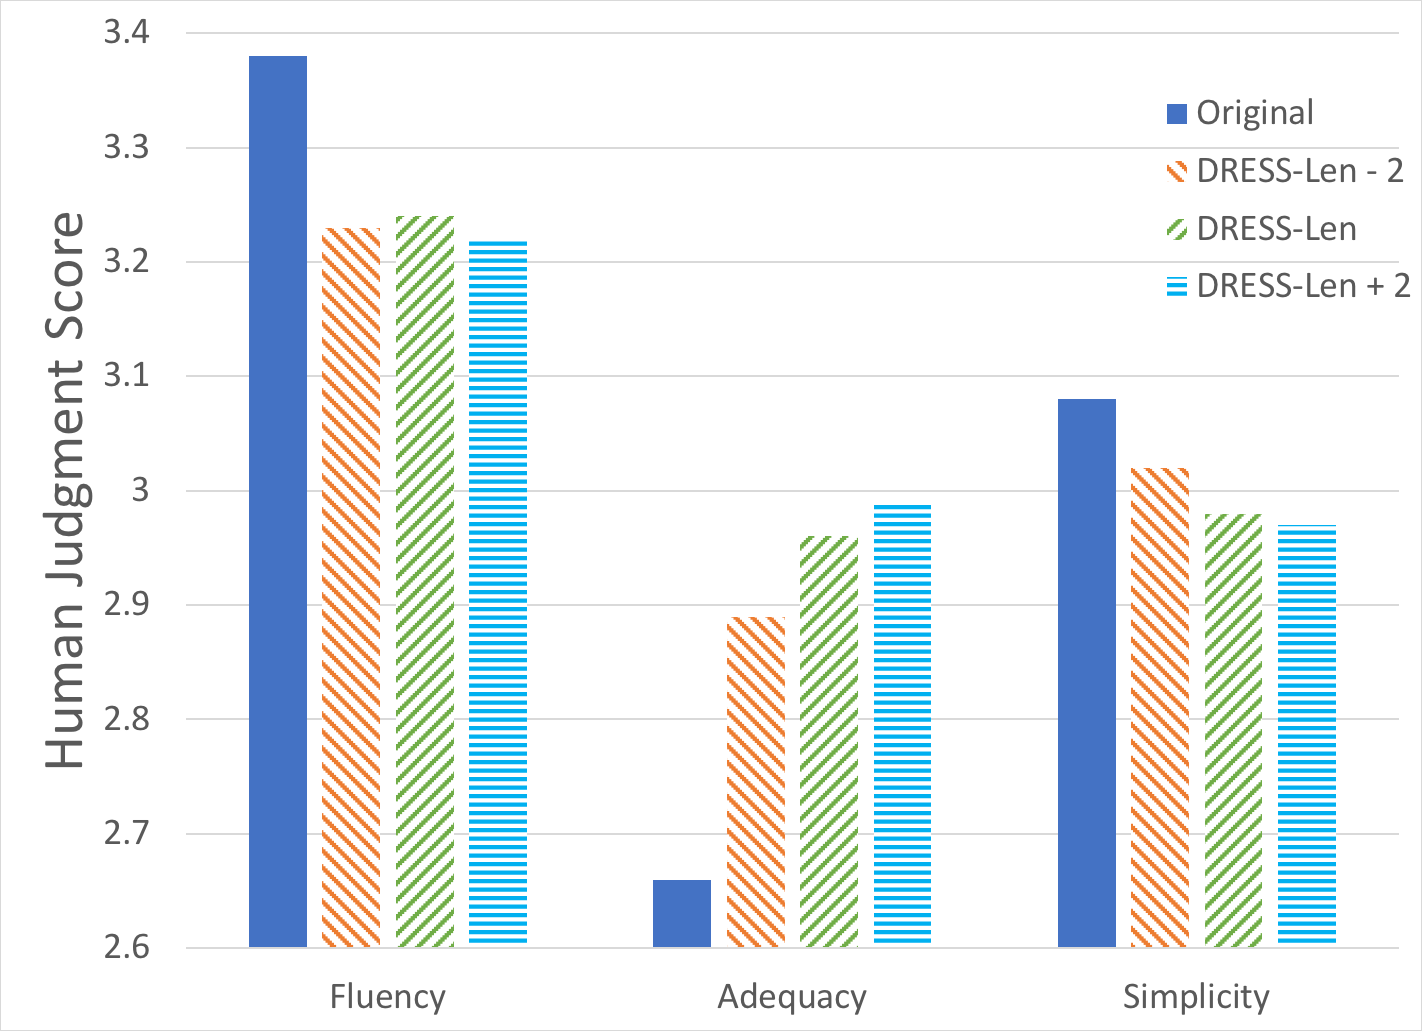
\includegraphics[width=7.5cm]{pictures/graph3.png}
\caption{Effect of length on human judgments.}
\label{length}
\end{figure}

The average fluency, adequacy, and simplicity from human judgments on these new sentences are shown in Figure \ref{length}, along with those ranked highest by our best model (Original). As expected, meaning preservation does substantially increase as we increase the average sentence length, while simplicity decreases. Interestingly, fluency also decreases as sentence length increases; this is likely due to our higher-ranked sentences having greater fluency, as defined by language model perplexity.

\subsubsection{Error Analysis} \label{sec:sentence_errors}

To gain insight in what aspects of the simplification process are challenging to our model, we present the most recurring types of errors from our test set.

\begin{enumerate}
\item{Long and complex sentences with multiple clauses}

\begin{enumerate}
\small
\item{\label{longandcomplex1}} \underline{\it Complex}: Turkey has long enshrined the secular ideals of founding father Mustafa Kemal Ataturk, particularly in an education system that until recently banned Islamic headscarves in schools and made schoolchildren begin the day reciting an oath of allegiance to Ataturk's legacy. \\
\underline{\it Reference}: Schools in Turkey had banned headscarves.\\
\underline{\it Simple}: They made schoolchildren to Ataturk's history.

\item{\label{longandcomplex2}} \underline{\it Complex}: And Wal-Mart, which imports more fruits and vegetables from Mexico than any other U.S. company, announced its effort to force improvements up and down its supply chain.\\
\underline{\it Reference}: Experts said Wal-Mart is an important company.\\
\underline{\it Simple}: Wal-Mart used more fruits and vegetables from the company.
\end{enumerate}

\item{Need for anaphora resolution}
\begin{enumerate}
\small
\item {\label{anaphoraresolution1}} \underline{\it Complex}: He is the creative director of Rethink Leisure \& Entertainment , which is working on several projects in China and elsewhere in Asia . \\
\underline{\it Reference}: He is with Rethink Leisure \& Entertainment.\\
\underline{\it Simple}: He is working on several projects in China.

\item {\label{anaphoraresolution2}} \underline{\it Complex}: Teachers there say Richie reads like a high school student.\\
\underline{\it Reference}: He reads like a high school student. \\
\underline{\it Simple}: Richie says he is a high school student.
\end{enumerate}

\item{Simplifying the wrong part of the sentence}
\begin{enumerate}
\small
\item{\label{wrongpart1}} \underline{\it Complex}: Parks deliberately maintained her image as shy and proper, said Adrienne Cannon, an expert on African-American history.\\
\underline{\it Reference}: Adrienne Cannon studies African-American history.\\
\underline{\it Simple}: She is an expert on African-American history.

\item{\label{wrongpart2}}\underline{\it Complex}: His father owned the home when the lava flowed slowly to the coast.\\
\underline{\it Reference}: His father still owned the home.\\
\underline{\it Simple}: The river cut slowly to the coast.\\
\end{enumerate}

\item{Poor substitution due to word embeddings proximity}
\begin{enumerate}
\small
\item{\label{badsub1}} \underline{\it Complex}: Just until recently, the education system had banned Islamic \textbf{headscarves} in schools and made schoolchildren begin the day reciting a pledge of allegiance to Ataturk's legacy.\\
\underline{\it Reference}: Schools in Turkey had banned headscarves.\\
\underline{\it Simple}: Just until recently, the education officials had banned  Islamic \textbf{flags}.
\item {\label{badsub2}} \underline{\it Complex}: In Beijing kite circles, Fei is widely known as the elder \textbf{statesman}.\\
\underline{\it Reference}: In Beijing, Fei is widely known as an expert.\\
\underline{\it Simple}: In Beijing, Fei is considered a \textbf{doctor}.
\end{enumerate}

\item{Training confusion due to misalignments in training corpus}
\begin{enumerate}
\small
\item {\label{badalignment1}} \underline{\it Complex}: He heard the applause.\\
\underline{\it Reference}: The winning word was ``magician."\\
\underline{\it Simple}: But he heard the song.

\item{\label{badalignment2}} \underline{\it Complex}: More than 300,000 students across the country signed up to participate. \\
\underline{\it Reference}: Rogers Middle School took part in the program.\\
\underline{\it Simple}: There were more than 300,000 students.
\end{enumerate}

\item{Acceptable simplifications that were not available in the training}
\begin{enumerate}
\small
\item{\label{acceptable1}} \underline{\it Complex}: He later tried to buy his freedom.\\
\underline{\it Reference}: Henson tried to buy his freedom later. \\
\underline{\it Simple}: The man tried to buy his freedom.

\item{\label{acceptable2}} \underline{\it Complex}: Middle school was a rough couple of years for Talmus' daughter, Lili Smith. \\
\underline{\it Reference}: She had a hard time in middle school.\\
\underline{\it Simple}: School was a rough couple of years.
\end{enumerate}
\end{enumerate}

Attempting to rewrite very long and complex sentences resulted to consistent errors, as shown in \ref{longandcomplex1} and \ref{longandcomplex2}. This observation in combination with the examples of mis-alignments in the training corpus (\ref{badalignment1} and \ref{badalignment2}) indicate that we either need to improve the alignments such the model can capture that the simplification process involves in many cases splitting a sentence and then simplifying or train to learn when to split first and then attempt rewriting. 

The next two types of errors show failure in capturing discourse level meaning: a) errors due to failed pronoun resolution, shown in \ref{anaphoraresolution1} and \ref{anaphoraresolution2}, and b) errors due to the most important part of the sentence being left out, shown in \ref{wrongpart2} and \ref{wrongpart2}. In these cases, the sentences were not bad, but the information was assigned to the wrong referent, or important meaning was left out. In \ref{badsub1} and \ref{badsub2}, the substitution is clearly semantically related to the target, but changes the meaning. Finally, there were examples of acceptable simplifications, as in \ref{acceptable1} and \ref{acceptable2}, that were classified as errors because they were not in the gold data. We provide additional examples for each error category in the appendix.

To improve the performance of future models, we see several options. We can improve the original alignments within the Newsela corpus, particularly in the case where sentences are split. Prior to simplification, we can use additional context around the sentences to perform anaphora resolution; at this point, we can also learn when to perform sentence splitting; this has been done in the Hybrid model \citep{narayan2014hybrid}, but has not yet been incorporated into neural models. Finally, we can use syntactic information to ensure the main clause of a sentence is not removed.

\section{Simple-QE: Better Automatic Quality Estimation for Text Simplification} \label{sec:simpleqe}

In many text generation tasks, it is generally necessary to evaluate model quality using human judgments. However, this is expensive and time consuming, and is untenable when testing many model variations. Thus, many works have attempted to develop metrics to automatically evaluate the quality of generation models. Previous evaluation metrics \citep{papineni2002bleu,xu2016optimizing} estimate the quality of generated texts by comparing them to human-written simplifications, which restricts their use to settings where such references are available. In addition, comparing simplifications to a single reference is often too restrictive, as most texts can be simplified in a variety of ways.

We propose a model for measuring the quality of automatically generated simplifications, which does not require human references. Our model, Simple-Quality Estimation (Simple-QE), adapts the BERT-based summary QE model Sum-QE \citep{xenouleas2019sumqe}, to the simplification setting. As opposed to summaries -- which contain specific pieces of information from the original text 
and omit unimportant passages -- simplified text typically expresses all the content present in the original text using simpler words and structures. Both types of text, however, need to fulfill some linguistic quality constraints in order to be useful, such as being  grammatical and well-formed. We show that Simple-QE correlates well with human judgments of linguistic quality on system output produced by simplification systems. In addition, we adapt our model to make reasonable complexity predictions at both the sentence and document level. Our models can be used to optimize both simplification system development and the process of writing manual simplifications.

\begin{figure*}[bt]
    \centering
    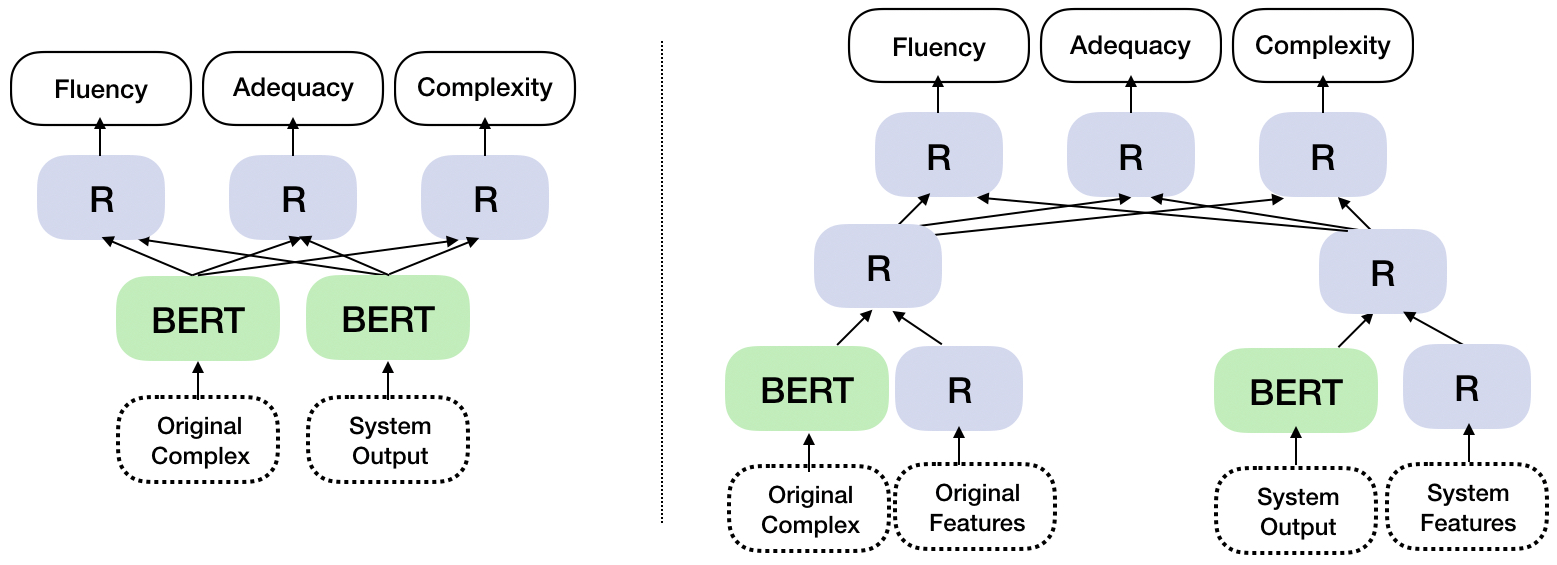
\includegraphics[width=11.5cm]{pictures/simpleQE_architecture.jpg}
\caption{The Simple-QE architecture, with and without adding numeric features corresponding to the original complex sentence (Original Features) and the system output (System Features). $R$ denotes a regressor layer.}
\label{fig:simpleqe-arch}
\end{figure*}

\subsection{Methodology} \label{sec:simpleqe-method}

To estimate the overall quality of a simplification system output, we focus on three linguistic aspects:

\begin{itemize}
    \item \textbf{Fluency}: How well-formed the system out is.
    \item \textbf{Adequacy}: How well the system output preserves the meaning of the original text.
    \item \textbf{Complexity}: How much 
    simpler the system out is than the original text. sentence.
\end{itemize} 

We adapt the architecture proposed by \cite{xenouleas2019sumqe} in their Sum-QE model, which extends the BERT fine-tuning process \citep{devlin2019bert} to rate summaries with respect to five linguistic qualities. We expect Fluency, in our setting, to align well with Grammaticality as addressed by Sum-QE. In the case of Adequacy and Complexity, since judgments are relative (e.g. is the generated text {\it simpler than} the original text? does it convey {\it the same} meaning?), we need to also consider the original complex text.

\cite{xenouleas2019sumqe} use BERT as the main encoder and fine-tune it in three ways, one single-task and two multi-task approaches:

\begin{itemize}
    \item \textbf{Single Task (S-1)}: Train $k$ models on each annotation type, where $k$ is the number of linguistic qualities; here, $k$ = 3.
    \item \textbf{Multi Task-1 (M-1)}: Train one model with a single regressor to predict $k$ annotations.
    \item \textbf{Multi Task-$k$ (M-3)}: Train one model with $k$ separate regressors, each corresponding to an individual annotation.
\end{itemize}

To adapt Sum-QE to simplification, we extend the architecture to take into account the original complex sentence. We do so by passing the original complex sentence and simplification system output through the BERT architecture separately. We concatenate the resulting embedding representations, and pass them through a final dense linear regressor layer $R$ to predict each linguistic quality score. Our adaptation of the Sum-QE Multi Task-3 (M-3) approach is described on the left side of Figure \ref{fig:simpleqe-arch}.

To further adapt the QE model to our task, we also attempt to incorporate task-specific features: the average {\bf Length} of content words in a sentence in characters and in {\bf Syllables}, their {\bf Unigram Frequency},\footnote{We use the average log unigram frequency from the Google $n$-gram corpus \citep{thorsten2006web}.} the {\bf Sentence Length}, and the syntactic {\bf Parse Height}. We pass these features extracted from the original complex sentence separately through a linear layer, before concatenating them with the BERT embeddings of the sentence. We do the same for the system output. The right side of Figure \ref{fig:simpleqe-arch} describes this architecture.

\subsection{QE Experiments on System Output} \label{sec:simpleqe-experiments}

Our test data consists of human judgments collected in Section \ref{paper:sentence_simplification} on generated simplifications for 200 Newsela sentences \citep{xu2015problems}. For each sentence, outputs from six simplification models were considered: vanilla Sequence-to-Sequence (Seq2Seq) \citep{nisioi2017exploring}, Seq2Seq with reinforcement learning \citep{zhang2017sentence}, memory-augmented Transformer \citep{zhao2018integrating}, and three variations of our Seq2Seq model with post-training re-ranking from Section \ref{sec:sentence}. Annotators were asked to rate the Fluency, Adequacy, and Complexity of each system output on a 5-point Likert Scale. Note that we do not use the QE dataset introduced by \cite{stajner2016quality}, as it focuses on small-scale lexical changes -- similar to the Turk dataset \citep{xu2016optimizing} -- while current neural models adopt a more holistic approach.

\begin{table*}
\begin{center}
\scalebox{0.90}{
\begin{tabular}{|c|c c c | c c c | c c c | } \hline
\multirow{2}{*}{\textbf{Model}} & \multicolumn{3}{|c|}{\textbf{Fluency}} & \multicolumn{3}{|c|}{\textbf{Adequacy}} & %\multicolumn{3}{|c|}{\textbf{Simplicity}}\\
\multicolumn{3}{|c|}{\textbf{Complexity}}\\
& $\rho$ & $\tau$ & $r$ & $\rho$ & $\tau$ & $r$ & $\rho$ & $\tau$ & $r$ \\ \hline
BLEU & 0.167 & 0.116 & 0.183 & 0.278 & 0.195 & 0.305 & 0.046 & 0.033 & 0.057 \\
SARI & 0.140 & 0.098 & 0.133 & 0.192 & 0.133 & 0.207 & 0.002 & 0.002 & 0.013 \\ \hline
BERT LM & 0.443 & 0.314 & 0.411 & 0.397 & 0.277 & 0.350 & 0.277 & 0.195 & 0.249 \\
BERT Sim & 0.288 & 0.202 & 0.278 & 0.530 & 0.382 & 0.533 & 0.095 & 0.066 & 0.085 \\ \hline
Sum-QE S-1 & 0.603 & 0.430 & 0.619 & 0.484 & 0.346 & 0.489 & 0.392 & 0.275 & 0.388 \\
Sum-QE M-1 & 0.626 & 0.446 & 0.632 & 0.535 & 0.384 & 0.541 & 0.403 & 0.282 & 0.407 \\
Sum-QE M-3 & 0.627 & 0.448 & 0.638 & 0.519 & 0.371 & 0.518 & 0.421 & 0.297 & 0.418 \\ \hline
Simple-QE S-1 & 0.619 & 0.443 & 0.635 & 0.545 & 0.393 & 0.549 & 0.438 & 0.309 & 0.436 \\
Simple-QE M-1 & 0.628 & 0.448 & 0.643 & \textbf{0.623} & \textbf{0.454} & \textbf{0.630} & 0.435 & 0.305 & 0.433 \\
Simple-QE M-3 & \textbf{0.638} & \textbf{0.459} & \textbf{0.648} & 0.604 & 0.439 & 0.612 & \textbf{0.459} & \textbf{0.325} & \textbf{0.464} \\ \hline
\end{tabular}
}
\end{center}
\caption{\label{SimpleQE-experiments} Correlations with human judgements on Fluency, Adequacy and Complexity of simplification system output; Spearman's $\rho$, Kendall's $\tau$ and Pearson's $r$ are reported.}
\end{table*}

We compare the Simple-QE model to baselines that use the simplification-specific features described in Section \ref{sec:simpleqe-method}, quality estimates provided by BLEU \citep{papineni2002bleu} and SARI \citep{xu2016optimizing}, and three additional BERT-based baselines.

\begin{itemize}
    \item \textbf{BERT as Language Model (BERT LM)}: Given a sentence, we mask each token and predict the likelihood of the true word occurring in this context; this captures Fluency.\footnote{https://github.com/xu-song/bert-as-language-model}
    \item \textbf{BERT embedding similarity (BERT Sim)}: We convert the original and simplified texts into sentence-level BERT vector representations via mean pooling, and compute their cosine similarity; this estimates Adequacy.
    \item \textbf{Sum-QE}: We apply Sum-QE directly, fine-tuning only on annotated system output.
\end{itemize}

For Sum-QE and Simple-QE, we perform 10-fold cross validation, combining the results to compute the overall correlation.

The results are shown in Table \ref{SimpleQE-experiments}. Simple-QE correlates better with human judgments than the baseline models tested. The correlation of BLEU and SARI with human judgments is particularly low, especially for Complexity. This is not surprising, given that SARI mainly addresses lexical simplification, while recent models approach simplification more holistically. 

The three versions of Simple-QE perform similar to Sum-QE on Fluency, where the model does not need to access the original complex sentence. The difference between the two models is more noticeable for Adequacy and Complexity, where accessing the original sentence actually helps Simple-QE make more reasonable 
estimates. From the three versions of Simple-QE tested, the multi-task versions perform better than the single task on all three qualities tested. The \textbf{BERT LM} and \textbf{BERT Sim} baselines perform well on Fluency and Adequacy, as expected, but fall short on the other aspects of simplification. As shown in Table \ref{SimpleQE-experiments}, adding numeric features do not improve performance. This may be because the most predictive features, e.g. sentence length, are already implicitly learned by BERT, as recent probing works have shown that the syntax of a sentence can be extracted from contextual word embeddings with reasonable accuracy \citep{hewitt2019structural}.

\section{Summary}

In this chapter, we first present a novel Seq2Seq framework for sentence simplification. We contribute three major improvements over generic Seq2Seq models: a complexity-weighted loss function to encourage the model to choose simpler words; a similarity penalty during inference and clustering post-inference, to generate candidate simplifications with significant differences; and a re-ranking system to select the simplification that promotes both fluency and adequacy. Our model outperforms previous state-of-the-art systems according to SARI, the standard metric for simplification used in our evaluation, while we highlight the issues with the current automatic metrics. More importantly, while previous models generate relatively long sentences, our model is able to generate shorter and simpler sentences, while remaining competitive regarding human-evaluated fluency and adequacy. Finally, we provide a qualitative analysis of the improvements introduced by our specific contributions, discuss the effect of sentence length on human-evaluated meaning preservation, and the shortcomings of our model as insights for future research.

In the second part of this chapter, we present Simple-QE, a quality estimation model for simplification. We have shown that extending Sum-QE \citep{xenouleas2019sumqe} to include the reference complex sentence significantly improves predictions on Adequacy and Complexity. QE systems can be useful for evaluating the overall quality of model output without requiring expensive human annotations or references. Future simplification systems can incorporate Simple-QE into the optimization process, similar to how SARI was incorporated into a Seq2Seq network \citep{zhang2017sentence}.

From the modifications we applied to standard Seq2Seq architectures, we found that the ones that improved performance on sentence simplification were incorporating a diverse decoding strategy, followed by re-ranking the resulting candidates. As we note, our methodology for sentence simplification is only one of many strategies that have recently been developed, as many open-ended language generation tasks can greatly benefit from multiple unique but valid candidate outputs. In the following chapter, we further pursue this idea of diversity, and perform an exhaustive comparison of current diverse decoding techniques on two tasks: conversational dialogue systems and image captioning. While these tasks have different goals than sentence simplification, all three fields share the fact that they benefit from re-ranking or combining diverse candidate outputs.

\biblio
\end{document}
